%latex slides_FMeot.tex  ; latex slides_FMeot.tex  ; dvips slides_FMeot.dvi ; dvipdf slides_FMeot.dvi 
\documentclass[12pt]{article}

%\usepackage{draftcopy}
%\usepackage[draft]{graphicx}
\usepackage{graphicx}
%\usepackage{wrapfig}
\usepackage{amssymb}
\usepackage{lscape}
\usepackage{times}
\usepackage{color}  % For \textcolor and \color % Ex. : \textcolor{red}{Text colored with} ; {\color{red}Text colored with}
\usepackage{soul}   % For \hl{ highlighted text} ; \sethlcolor{colorname}
%\usepackage[table]{xcolor}
\usepackage{xcolor,colortbl}
\usepackage{yfonts}  % for textgoth

%   portrait
%\oddsidemargin =-0.4in
%\evensidemargin=-0.4in
%\textwidth=6.8in
%\textheight=8in
%\topmargin=-1.in
%\footskip=0in
%   landscape
 \oddsidemargin =-.8in                            
 \evensidemargin=-.8in                                                          
 \textwidth=8.1in              
 \textheight=10.1in                       
 \topmargin=-.9in
 \footskip=-0in                                                                   

\newcommand{\Br}{\ensuremath{B\!\rho}}
\newcommand{\bull}{\ensuremath{\bullet~}}
\newcommand{\Bz}{\ensuremath{{B_z}}}
\newcommand{\CE}{concentration ellipse}
\newcommand{\CES}{CE-$\mathcal{S}$}
\newcommand{\com}{{center of mass}}
\newcommand{\dEE}{\small \ensuremath{\frac{dE}{E}}}
\newcommand{\dip}{\textit{ DIPOLE}}
\newcommand{\eg}{\textsl{e.g.}}
\newcommand{\ie}{\textsl{i.e.}}
\newcommand{\EFB}{\ensuremath{E\!F\!B}}
\newcommand{\EFBs}{\ensuremath{E\!F\!B\!s}}
\newcommand{\ffag}{\textit{ FFAG}}
\newcommand{\hel}{\ensuremath{\mathbf{^3 H\! e ^{2+}}}}
\newcommand{\hbrk}{\hfill \break}
\newcommand{\x}{\ensuremath{x}} 
\newcommand{\xp}{\ensuremath{{x'}}}
\newcommand{\y}{\ensuremath{y} }
\newcommand{\yp}{\ensuremath{{y'}}}
\newcommand{\dl}{\ensuremath{{\delta l}}} 
\newcommand{\lab}{\ensuremath{lab. frame}}
\newcommand{\MC}{Monte~Carlo}
\newcommand{\nib}{\noindent \ensuremath{\bullet}~}
\newcommand{\snib}{\noindent {\small \ensuremath{\bullet}}~}
\newcommand{\nid}{\noindent \ensuremath{\diamond}~}
\newcommand{\snid}{\noindent {\small \ensuremath{\diamond}}~}
\newcommand{\sid}{{\small \ensuremath{\diamond}}~}
\newcommand{\nin}{\noindent~}
\newcommand{\p}{\ensuremath{\mathbf{p}}}
\newcommand{\pp}{$p\! \! \uparrow$}
\newcommand{\rms}{\ensuremath{rms}}
\newcommand{\SRl}{SR loss}
\newcommand{\Sx}{\ensuremath{\mathcal{S}_x}}
\newcommand{\Sy}{\ensuremath{\mathcal{S}_y}}
\newcommand{\Sz}{\ensuremath{\mathcal{S}_z}}
\newcommand{\wrt}{{with respect to}}
\newcommand{\Y}{\ensuremath{Y} }
\newcommand{\Yp}{\ensuremath{{Y'}}}
\newcommand{\z}{Zgoubi}


\newcommand{\C}{\ensuremath{\mathcal{C}}}
\newcommand{\D}{\ensuremath{\mathcal{D}}}
\newcommand{\HH}{\ensuremath{\mathcal{H}}}
\newcommand{\bHH}{\bar \HH}
\newcommand{\LL}{\ensuremath{\mathcal{L}}}
\newcommand{\zg}{Zgoubi}

\newcommand{\black}{\color{black}}
\newcommand{\red}{\color{red}}
\newcommand{\green}{\color{green}}
\newcommand{\blue}{\color{blue}}
\newcommand{\BurntOrange}{\color{BurntOrange}}

\newcommand{\hlyell}[1]{{\sethlcolor{yellow}\hl{#1}}}
\newcommand{\hlcyan}[1]{{\sethlcolor{cyan}\hl{#1}}}

\newcolumntype{a}{>{\columncolor{gray!40!white}}c}
\newcolumntype{b}{>{\columncolor{blue!10!white}}c}

\definecolor{yell80}{rgb}{1,1,.8}
\definecolor{yell60}{rgb}{1,1,.6}
\definecolor{yell40}{rgb}{1,1,.4}
\definecolor{yell20}{rgb}{1,1,.2}
\definecolor{bluelight}{rgb}{.75,.946,1.}
\newcommand{\referenceA}{\rm  }
\newcommand{\referenceB}{\rm }
\newcommand{\referenceC}{\rm }



\pagestyle{myheadings}

\markboth
%{\Huge \red ~�\large  }
%{\Huge \red ~�\large  }
{\it \red ~�\large  ACCELERATORS, A Speed-of-Light Universe, Dpt. of Physics and Astronomy, SBU-SUNY - 2017}
{\it \red ~�\large  ACCELERATORS, A Speed-of-Light Universe, Dpt. of Physics and Astronomy, SBU-SUNY - 2017}


\begin{document}
\landscape

\title{
\fontsize{33pt}{34pt}\selectfont \it \blue
ACCELERATORS \\ A Speed-of-Light Universe \\ Dpt. of Physics and Astronomy, SBU-SUNY \\ 2017 \\[5ex]
\fontsize{29pt}{34pt}\selectfont \bf \black
\fbox{ Fixed Field Alternating Gradient Synchrotrons }
}

\thispagestyle{empty}



\author{ 
~
\\[5ex]
\fontsize{29pt}{34pt}\selectfont \bf
 Fran\c{c}ois~M\'eot \\
~ \\
\fontsize{29pt}{34pt}\selectfont \rm
Brookhaven National Laboratory \\
\fontsize{29pt}{34pt}\selectfont 
Collider-Accelerator Department \\
\fontsize{29pt}{34pt}\selectfont 
 Upton, LI, NY
}


\date{}


\thispagestyle{empty}

\maketitle

\clearpage

\tableofcontents




\clearpage



\sffamily

\section*{\LARGE Introduction}

\begin{minipage}[b]{.45\linewidth}
\Large

Only 5 FFAG machines  operated~:     

- 3 electron machines by the MURA Lab.,  50's

- 2 proton machines by KEK,  these last years 

- nevertheless,  FFAG have often been proposed as alternative solutions 
for the production of proton beams
%synchrotrons as p-drivers,  high power machines (e or p), 
%and for fast acceleration (muons), etc.

- more recently, the neutrino factory studies triggered strong R\&D activity. 

New concepts, new technologies reactivate the interest in the method. 


~~~~~~~~~~~~~~~~~~~~

~~~~~~~~~~~~~~~~~~~~

%{\it ``S'il te plait, dessine-moi une fleur''\\
%After Antoine de St-Exupery, Le petit Prince.}

~~~~~~~~~~~~~~~~~~~~

~~~~~~~~~~~~~~~~~~~~
% Invention by Simon/Ohkawa. Spiral optics invented by Kerst

\end{minipage}\hspace{0mm}
\begin{minipage}[b]{.65\linewidth}

\vspace{-17mm}

\hspace{20mm} 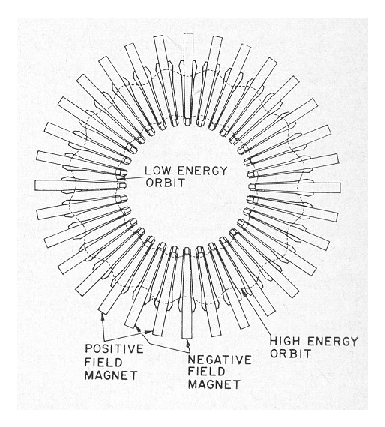
\includegraphics[width=12.cm]{./figures/ring3Draw.eps}

\vspace{-10mm}
\begin{center} \Large  The  MURA 2-way FFAG \\
Fundamental ingredients~: \\
fixed  field, 
strong focusing, synchrotron stability.  
% \\
%Specific to FFAG~: scaling, i.e. replication of  \\ orbits and optical functions. 
\end{center}
\end{minipage}



\clearpage 

\section{\LARGE  MURA electron FFAGs }

\large  

%http://www.fnal.gov/pub/about/whatis/timeline.html
%1952: MURA, the Midwestern Universities Research Association, is formed with 
%the goal of designing the next large U.S. accelerator facility. 
%1959: MURA considers the conceptual design of a several-hundred GeV machine, 
%including Robert Wilson's idea of cascading accelerators. 
%The MURA Lab.  formed in 1953 -  remember the context in these years~: 
%- the dead-end in energy  of the weak-focusing concept 
%- strong focusing has just been invented by CLS (1952) and  Christophilos (patent dates from 1954)
%- separate function (bending and focusing) proposed in  1953

\subsection*{\Large     The first model, radial sector FFAG, Mark II}

\large   

Objectives~:  confirm theoretical predictions~; study FFAG  properties~: optics, injection, test RF programs~; 
effects of misalignements~; effects  of resonances. 


\begin{minipage}[b]{.26\linewidth}
%\begin{center}  
%\hspace{-20mm} \includegraphics*[bbllx=60,bblly=60,bburx=245,bbury=230,width=10.cm]{./figures/drawRing1.eps}
\hspace{-7mm}  \includegraphics*[bbllx=40,bblly=50,bburx=440,bbury=350,width=7.5cm]{./figures/ring1Photo.eps}

\smallskip
\hspace{-3mm} \includegraphics*[bbllx=90,bblly=130,bburx=760,bbury=440,width=6.5cm]{./figures/ring1MagPhoto.eps} 

\hspace{-3mm} \includegraphics*[bbllx=14,bblly=14,bburx=450,bbury=200,width=6.5cm]{./figures/ring1MagDraw.eps}

\vspace{-5mm}
\begin{center}  
F magnet, positive field, radially focusing.  
 \end{center}


~~~~~~~~~~~~~

~~~~~~~~~~~~~
\end{minipage}\hspace{1mm}
\begin{minipage}[b]{.65\linewidth}
\large   
First operation March 1956, U of Michigan. 

\vspace{-5mm}
  \begin{center}
   \begin{tabular}{llccc}
\multicolumn{4}{c}{Machine parameters}    &        criteria / comments  \\[2mm]
&$E_{inj} - E_{max}$&\it keV&    25 - 400      & \bigg\{\raisebox{1ex}[0mm][0mm]{\it small size, easy to build ~~ ~ ~~ ~ ~~}  \\
      & orbit radius  ($\mathcal{C}/2\pi$) &\it m&0.34 - 0.50&\raisebox{2ex}[0mm][0mm]{\it field not too low, ms lifetime }   \\
\\[-2ex]
\multicolumn{2}{l}{\it \underline{Optics}}   \\
      & lattice    &     &$\mathbf{ \frac{D}{2} F\frac{D}{2}}$&   \\
      & number of cells& &       8           &  \it 16 magnets \& 4.41 deg. drifts\\
      &field index $K$&  &      3.36         &  \it $g/r=$Cst  \& pole-face windings         \\
      &$\nu_r~/~\nu_z$&  &   2.2-3 ~/~ 1-3   & \bigg\{  \raisebox{1ex}[0mm][0mm]{\it varying K, resp. $B_F/B_D$~~}  \\
      &            &     &              &\raisebox{2ex}[0mm][0mm]{\it varies  mostly  $\nu_r$, resp. $\nu_z$}\\[-2ex]
      &  $\gamma_t$ &  &     $\approx 2$  &       \it  $\sqrt{1+K}$  \\
\\[-2ex]
\multicolumn{2}{l}{\it \underline{Magnet}}&  \multicolumn{2}{c}{radial sector} & \it  $B=B_0 (r/r_0)^K \, F(\theta)$ \\
&$\theta_F,~ \theta_{D}$&\it deg&    25.74, ~ 10.44 &  \it sector angles        \\ 
      &  $r_{F,D}/\rho$& &     2.85, ~ 2.59  &   \it at center of F, D magnets       \\
      &   gap      &\it cm  &     6 - 4          &   \it $g/r=$Cst  \\     \\
\\[-3ex]
\multicolumn{2}{l}{\it  \underline{Injection}}&  \multicolumn{2}{c}{continuous or pulsed }  \\
\\[-1.5ex]
\multicolumn{2}{l}{\it  \underline{Acceleration}}& \multicolumn{2}{c}{ only betatron, at first...   }         &   \it for simplicity \\
      & swing  &\it  Gauss &   40 - 150   &  \\
      & rep. rate&\it Hz&      \textsf{a few 10's}          &       \\
\multicolumn{2}{l}{\it }& \multicolumn{2}{c}{... completed with RF acc., next   }  &  \it split tank  \\
      & freq. swing&\it MHz &  10\textsf{~in}~ [35,~75]~\textsf{MHz}  &  \it  for  RF stacking expts\\
      & gap voltage&\it V  &        50         &  \\
      &cycle rep. rate&\it kHz&      \textsf{a few}          &  \it to cope with lifetime    
   \end{tabular}
  \end{center}

~~~~~~~~~~~~~

\end{minipage}




\clearpage 

\subsection*{\Large   How this works...  }

\large 

\hspace{-8mm}
\begin{minipage}[b]{.70\linewidth}
\begin{itemize}
  \item Magnetic field is fixed in time, and  fast increasing with radius,
 {\Large$B=B_0 (\frac{r}{r_0})^K $ }
  \vspace{-7mm}
  \begin{itemize}
    \item from   lower energy  on inner orbit
    \item to largest energy on outer orbit
  \end{itemize}
  \item Transverse motion stability is ensured by AG focussing
  \vspace{-2mm}
  \begin{itemize}
    \item {\it \Large Strong} focusing, as in pulsed synchrotrons, hence small beta functions
    \item AG is obtained by alternance of 
    \begin{itemize}
      \item positive curvature field sectors, hence focussing, {\Large $\frac{\rho(s)}{B(s)}\, \frac{dB}{d\rho} >0$}
      \item negative curvature field sectors, hence defocussing, {\Large $\frac{\rho(s)}{B(s)}\, \frac{dB}{d\rho} <0$}
      \item with ratio {\Large $|\int B_D \, ds| \approx \frac{2}{3} \times \int B_F \, ds$},  to ensure axial focussing
    \end{itemize}
  \end{itemize}
  \item  The  radial dependence {\Large  $B=B_0 (r/r_0)^K $} yields the 
  {\it \Large scaling} property~:
  \vspace{-3mm}
  \begin{itemize}
    \item orbits are similar wrt. geometrical center
    \item tunes  are independent of  orbit 
  \end{itemize}
  \item Corollaries
  \vspace{-2mm}
  \begin{itemize}
%    \item $\alpha = 1 / (1+K)$ 
    \item  large {\it \Large circumference factor}~~ {\Large $\mathcal{C}/2 \pi \rho$  } due to alternating curvature
    \item drift length is not free
%    \item scalloping is small~: orbit length = $r \times (2 \pi+\epsilon) $, $\epsilon$ small 
    \item {\Large $\alpha = 1/(1+K) \rightarrow$} larger K ensures smaller {\Large $r_{max}-r_{min}$}
    \item transition energy  $E_{tr} = E_0/ \sqrt{\alpha} \approx E_0 \sqrt{1+K}$ easily beyond $E_{max}$
    \item etc.
  \end{itemize}
  \item Longitudinal motion~: satisfies phase stability concepts
  \vspace{-2mm}
  \begin{itemize}
    \item sophisticated RF programs are possible~: $\omega_{RF}$ does not  track B
    \item extremely high average gradients  are possible 
  \end{itemize}
\end{itemize}
\end{minipage}\hspace{-5mm}
\begin{minipage}[b]{.5\linewidth}\hspace{3mm}
%\begin{center}
\includegraphics*[bbllx=34,bblly=70,bburx=245,bbury=220,width=9cm]{./figures/ring1Draw.eps}

\hspace{2cm}\includegraphics*[bbllx=14,bblly=14,bburx=278,bbury=260,width=7cm, height=4cm]{./figures/fieldMarkI.eps}

\mbox{
\includegraphics*[bbllx=0,bblly=100,bburx=252,bbury=323,width=5cm]{./figures/geometry.eps}\hspace{-5mm}
\includegraphics*[bbllx=0,bblly=100,bburx=252,bbury=323,width=5cm]{./figures/geometryD.eps} 
}


\mbox{\hspace{3mm}
\includegraphics*[bbllx=0,bblly=0,bburx=300,bbury=254,width=4cm]{./figures/fFoc.eps}  \hspace{5mm}
\includegraphics*[bbllx=0,bblly=0,bburx=300,bbury=254,width=4cm]{./figures/dFoc.eps}
}

%\end{center}


\end{minipage}



\clearpage 

\subsection*{\Large  Linear optics  approximate methods }

\large 

%\begin{itemize}
%  \item Synchrotron motion~: as in AG synchrotron
%  \begin{itemize}
%    \item {\it the  theory assumes} as well acceleration  slow enough that one can consider  $B=C^{te}$ 
%over a  turn
%  \end{itemize}
%  \item Frequency program can be aritrary~: not constrained by B(t)
%\end{itemize}
\begin{center}
First ~: find the closed orbit {\Large $\leftarrow$} from  the FFAG parameters. 

\medskip
\hspace{-20mm} Then apply  (approximation)  the linear equations of motion about a closed orbit  

\medskip
{\LARGE ~ ~ ~ ~ ~ ~  ~ ~ ~ ~ ~ $ x'' + \frac{1-n}{\rho^2} x = 0, ~~~ z'' + \frac{n}{\rho^2} z = 0$}
~ ~ ~ ~ ~ ~ ~ ~ ~ ~~ ~ ~ ~ ~ ~ ~
\raisebox{7mm}[0mm][0mm]{\includegraphics*[bbllx=20,bblly=100,bburx=560,bbury=460,width=4cm]{./figures/envX.eps}}

\medskip
with ~ ~ ~ ~ ~ ~ ~  {\Large $~~~~ n(s)=-\frac{\rho(s)}{B(s)}\, \frac{dB}{dx} \approx -\frac{\rho}{B}\, 
\frac{dB}{dr} ~~~~ $}  (scalloping is negligible)
~ ~ ~ ~ ~ ~ ~ ~ ~ ~\raisebox{-8mm}[0mm][0mm]{\includegraphics*[bbllx=20,bblly=100,bburx=560,bbury=460,width=4cm]{./figures/envZ.eps}}
\medskip

The index $n(s)$ in the equations of motion, and $K$ in {\Large $B = B_0 (\frac{r}{r_0})^K$ } can be related as follows:

\medskip
{\Large $   \frac{dB}{dr} = K \frac{B_0}{r_0}  (\frac{r}{r_0})^{K-1}  = K \frac{B }{ R} 
~~~~$} \textsf{so that} {\Large $~~~~ \frac{r}{B} \frac{dB}{dr} =$ \fbox{$ K = -n C$}}. 

\smallskip
Equivalently  the  matrix representing a sector has the form
%\begin{equation}
{\Large $M= \left[ \begin{array}{cc}
 \cos(s \sqrt{k}) &  \frac{1}{\sqrt{k}} \sin(s \sqrt{k}) \\
 -\sqrt{k} \sin(s \sqrt{k})  & \cos(s \sqrt{k}) 
\end{array} \right]$  }           \\
%\end{equation}
%  with {\Large $k=\frac{1-n}{\rho^2}$} (radial motion) or {\Large $k=\frac{n}{\rho^2}$ } (vertical motion)
\smallskip
  with {\Large $k=(1-n)/\rho^2$} (radial motion) or {\Large $k=n / \rho^2$ } (vertical motion)

  \bigskip

The geometry provides the wedge angles and thus the wedge matrices, $M_{Fe1}$, $M_{Fe2}$, $M_{De1}$, $M_{2e2}$  

  \bigskip

The  product matrix  representing  a  D-F sector  yields the phase advance~: 

\medskip
{\Large $ \cos(\mu) = \frac{1}{2}Tr(M_{Fe2}\times M_F\times M_{Fe1}\times M_{De2} \times M_D\times M_{De1})/2$ ,...
}


\medskip

\rule{30mm}{.1mm}
\bigskip

The longitudinal motion in presence of RF acceleration satisfies 

\medskip
{\Large ~ ~ ~ ~ ~ ~ ~ ~ ~ ~ ~ ~  %\fbox{ 
$ \phi'' + \frac{\Omega^2}{\cos{\phi_s}}(\sin\phi - \sin \phi_s)=0$}
~ ~ ~ 
\raisebox{-10mm}[0mm][0mm]{\includegraphics*[bbllx=20,bblly=100,bburx=560,bbury=460,width=4cm]{./figures/synMot100MeV.eps}}

\medskip
yielding  classical results as \\
synchrotron frequency {\Large $f_s = \Omega_s/2\pi = \frac{c}{\mathcal{L}}\left( 
\frac{h \eta  \cos\phi_s q\hat{V}}{2 \pi E_s}\right)^{1/2}$~, } 
%, given $h=1$, $\phi_s=0$, $q\hat{V}=0.019$~MeV~; 
%$E_s$ is total energy and $T_{rev}$ and $\mathcal{L}$ are obtained by tracking (Tab.~\ref{TabParam150}),  
 bucket height  {\Large $\pm \frac{\Delta p}{p} = \pm \frac{1}{\beta_s} 
\left(\frac{ 2 q\hat{V}}{\pi h \eta E_s}\right)^{1/2}$ ,}      ~~  etc.

\end{center}


%``By virtue of its essential simplicity, the reversed-field type FFAG may remain of interest for 
%accelerators of low or intermediate energy, especially if a high duty-factor can be efficiently realized \[...\]''



\clearpage 

\subsection*{\Large  Second model, spiral sector FFAG, Mark V}

\large     

Interest of spiral optics~: always positive curvature, hence smaller accelerator,  compared to radial sector. 

\noindent Study objectives~:  confirm theoretical predictions - first extensive use of computers to determine 
magnetic field  and machine  parameters~; long-term orbit stability~; RF acceleration methods. 


\begin{minipage}[b]{.33\linewidth}
\hspace{-7mm} \includegraphics*[bbllx=14,bblly=14,bburx=250,bbury=220,width=9.cm]{./figures/ringSpiralDraw.eps}

\medskip
\includegraphics*[bbllx=14,bblly=44,bburx=250,bbury=230,width=4.5cm]{./figures/ringSpiralMagDraw.eps}

\includegraphics*[bbllx=14,bblly=44,bburx=278,bbury=195,width=5.5cm]{./figures/ringSpiralCoilDraw.eps}
  \begin{center}   Logarithmic spiral poles \end{center}

\end{minipage}\hspace{0mm}
\begin{minipage}[b]{.65\linewidth}
\large   

First operation Aug.~1957 at the  MURA Lab., Madison. 

  \begin{center}
   \begin{tabular}{llccc}
\multicolumn{4}{c}{Machine parameters}    &        criteria / comments  \\[2mm]
&$E_{inj} - E_{max}$&\it keV &    35 - 180      & \bigg\{ \raisebox{1ex}[0mm][0mm]{\it reasonable size}  \\
      &             &     &                  &  \raisebox{2ex}[0mm][0mm]{\it  magnets}   \\[-2ex]
      &orbit radius &\it  m   &   0.34 - 0.52   &  \\
      &$E_{tr}~/~r_{tr}$&\it keV~/~m&   155~/~0.49      &  \bigg\{ \raisebox{1ex}[0mm][0mm]{\it RF exprmnts ~~~~ ~ ~ ~~~ } \\
      &                &  &                  &   \raisebox{2ex}[0mm][0mm]{\it  at  $\gamma_{tr} =(1+K)^{1/2}$ }     \\[-2ex]
\\[-1.50ex]
\multicolumn{2}{l}{\it \underline{Optics}}   \\
      & lattice    &     &    N  spiral sectors  &   \\
      & number of sectors& &       6           &  \\[-.5ex]
      & field index $K$&  &      0.7          &   \bigg\{ \raisebox{1ex}[0mm][0mm]{\it pole-face windings, }  \\
      &                &  &                   &    \raisebox{2ex}[0mm][0mm]{\it  tunable 0.2-1.16  }       \\[-2ex]
      & flutter $F_{eff}$ &     &       1.1          &  \it tuning coils / 0.57 - 1.60 \\
      &$\nu_r~/~\nu_z$&  &   1.4~/~1.2       &  \it tunable  \\
      &$\beta_r ~/~ \beta_z$&\it m  &   0.45-1.3~/~0.6-1.4       &   \it  min-max  \\
\\[-1.50ex]
\multicolumn{2}{l}{\it \underline{Magnet}}&& spiral sector &\it $B$=$B_0 (\frac{r}{r_0})^K \, F(\ln \frac{r}{r_0}/w - N \theta)$ \\
      &  $1/w$       &     &       6.25          &   \it $2 \pi w r_0\approx$ ridges radial separation \\
      &  $\alpha=Arctg(Nw)$&\it deg&  46       &  \it edge to radius angle  \\
      &  $r_{min} - r_{max}$&\it m&    0.25 - 0.61  &  \\
      &   gap      &\it cm  &      16.5  - 7     &   \it $g/r=$Cte  \\
\\[-1.50ex]
\multicolumn{2}{l}{\it  \underline{Injection}}&   &cont. or pulsed &  \it e-gun + e-inflector \\
\\[-1.50ex]
\multicolumn{2}{l}{\it  \underline{Acceleration}}&&    \sf betatron and RF   & \it extensive RF prog. tests   \\
%      & RF  voltage&\it V  &        150         &  \\
   \end{tabular}
  \end{center}

~~~~~~~~~~~~~~~

~~~~~~~~~~~~~~~

~~~~~~~~~~~~~~~

~~~~~~~~~~~~~~~

~~~~~~~~~~~~~~~

\end{minipage}




\clearpage 

\subsection*{\Large   Optics  of the spiral FFAG }

\large \sf 

The idea in the spiral FFAG was to superpose a positive field on top of the alternating sign one of the 
radial sector, so as to always have the right curvature and thus decrease the circumference factor. 


\begin{minipage}[b]{.6\linewidth}

\large \sf 

The following form for the field preserves the scaling property in the spiral FFAG: 

{\Large $$   B(r, \theta)|_{z=0} = B_0 \left( \frac{r}{r_0} \right)^K \ 
\mathcal{F}\left(\ln \frac{r}{r_0}/w - N \theta \right) $$}

\medskip
$\mathcal{F}$ is the axial modulation of the field (``flutter''). One can for instance think of (not the best 
optics, though) $\mathcal{F}=1+f\sin(\ln \frac{r}{r_0}/w - N \theta)$. 

\medskip
The logarythmic spiral edge %{\Large ~ ~ $r = r_0 \exp(Nw \theta)$~ ~}
 ensures constant  angle (the ``wedge angle'') between  spiral sector edges and closed orbits. 

%\medskip
%The modulation is $2\pi/N$-periodic, a particle passes N ridges over a turn. 


\medskip
%In a simpler hard-edge model, 
%the optical ingredients to describe the closed orbit would be  the sector angle $\theta$ between edges, arc length $s$ and 
%curvature radius $\rho$,  the  index $n=-K\rho/R$ provides  
%the $\left( \begin{array}{cc} C & S \\ C' & S'\end{array} \right)$ matrix, 
%the wedge angle $\epsilon$ provides  the wedge matrices. 

%The half trace of the resulting product matrix yields

Expansion of the equations of motion around the scalloped orbit in the linear approximation  yields the tunes 
{\Large $$\nu_r \approx \sqrt{1 + K} , ~ ~ ~  \nu_z \approx  \sqrt{-K + (f/Nw)^2/2}$$  }

A matrix model using hard-edge approximation would give similar result to first order in the deviation. 


\end{minipage}\hspace{3mm}
\begin{minipage}[b]{.6\linewidth}

\vspace{-10mm}
\includegraphics[bbllx=90,bblly=0,bburx=500,bbury=460,width=10.cm]{./figures/spiral3D.eps}

\vspace{-20mm}
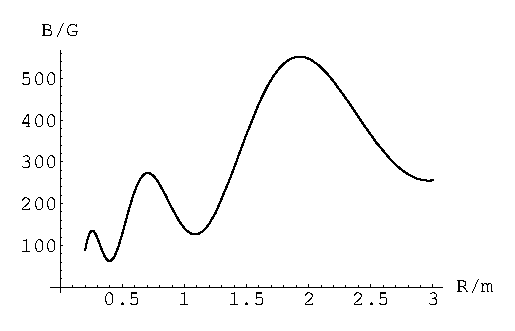
\includegraphics[width=10.cm,height=3cm]{./figures/spiralBvsR.eps}

\vspace{-10mm}
 \hspace{10mm}\includegraphics*[bbllx=14,bblly=120,bburx=520,bbury=500,width=8.cm]{./figures/spiralFoc.eps}

\end{minipage}




\clearpage 

\subsection*{\Large  Second radial sector FFAG, 50~MeV,  2-way}

\large   

Preliminary studies early 1957. The spiral sector e-model was not yet completed - this determinied the choice of radial sector~:  
easier to design, better understood.  

Study objectives~: ~~ 1/ RF stacking, ~~ 2/ high circulating $I$, ~~ 3/ 2-way storage. 

First start Dec.~1959, 2-beam mode, 27~MeV~; disassembled in 60, magnets corrected~;  second start Aug.~61, single beam, 50~MeV. 

\begin{minipage}[b]{.38\linewidth}
\hspace{-10mm} 
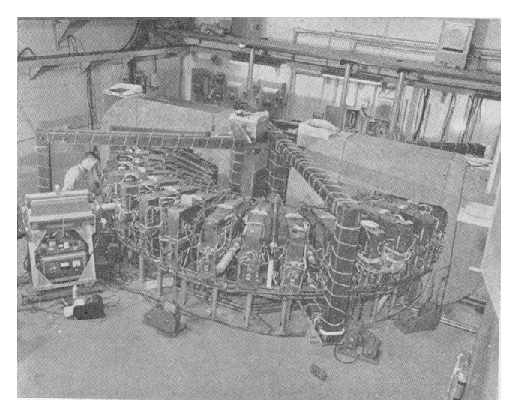
\includegraphics[width=16.cm]{./figures/photoRing.eps}

\vspace{-30mm}
\hspace{-7mm} \includegraphics*[bbllx=125,bblly=80,bburx=280,bbury=208,width=7.cm]{./figures/ring3Traj2way.eps} 
                                     \hspace{-10mm} {\Large\bf $B_F=B_D$ }\\
\end{minipage}\hspace{0mm}
\begin{minipage}[b]{.65\linewidth}
\large   
  \begin{center}
                   {\bf \Large   \underline{[Typical] data}} 
   \begin{tabular}{llccc}
\\[-3mm]
\multicolumn{4}{c}{Machine parameters}    &         criteria / comments  \\[2mm]
      & \bf $E_{inj} - E_{max}$  & \it     MeV  & \bf    0.1 - 50     & \bf     \it reasonable size \& beam life-time         \\
      & \bf orbit radius& \it  m   & \bf     1.20 - 2.00    & \bf           \\
\multicolumn{2}{l}{\it \underline{Optics}}   \\
      & \bf  lattice    &       & \bf    FODO            & \it $B\approx B_0(r/r_0)^K\, \cos(16\, \theta)$    \\
      & \bf  number of cells&   & \bf      16            & \bf      \it 32 magnets, 3.15~deg. drifts     \\
      & \bf    K        &       & \bf       9.25         & \bf             \\
      & \bf $\nu_r~/~\nu_z$&    & \bf     4.42~/~2.75    & \bf         \\[1ex]
%      & \bf  radial accept. & \bf  $\pi$cm & \bf    0.4    & \bf   \raisebox{1ex}[0mm][0mm]{\it mechanical limit is}  \\
%      & \bf             & \bf      & \bf                   & \bf   \raisebox{2ex}[0mm][0mm]{\it injection inflector}   \\[-2ex]
%      & \bf  vertical accept. & \bf  $\pi$cm & \bf    \\
\multicolumn{2}{l}{\it  \underline{Magnet}}  & \bf  & \bf  radial sector &\\
& \bf    $\theta$, core & \it  deg & \bf         6.3       & \bf           \\ 
      & \bf  peak field & \it  T   & \bf        0.52       & \bf    \it  $ r_{max}$       \\
      & \bf    gap      & \it  cm  & \bf        8.6        & \bf                    \\
      & \bf   power     & \it  kW  & \bf        100        & \bf              \\
\multicolumn{2}{l}{\it  \underline{Injection}}& \bf  & \bf & \it e-gun + e-inflector \\
\multicolumn{2}{l}{\it  \underline{Acceleration}}& \bf & \bf                 &  \\
      & \bf  swing      & \it  MHz & \bf    20 - 23   & \bf   \\
      & \bf harmonic    & \it      & \bf           1       & \bf   \\
      & \bf voltage p-to-p& \it  kV& \bf    1.3 - 3        & \bf   \\
%      & \bf    $\phi_s$ & \it  deg & \bf        20         & \bf          \\
%      & \bf    $\nu_s$  & \it      & \bf     0.039 - 0.012       & \bf        \\
      & \bf cycle rep. rate& \it Hz& \bf        60       & \bf       \\
   \end{tabular}
  \end{center}

~~~~~~~~~

\end{minipage}



%\clearpage


\large     

\begin{minipage}[b]{.3\linewidth}

\hspace{-20mm} \includegraphics*[bbllx=0,bblly=0,bburx=1024,bbury=768,width=9.cm]{./figures/PoPFFAG.eps}

\vspace{-70mm} \hspace{-20mm}\includegraphics[width=4.cm]{./figures/popMagnet.eps}

\vspace{40mm}

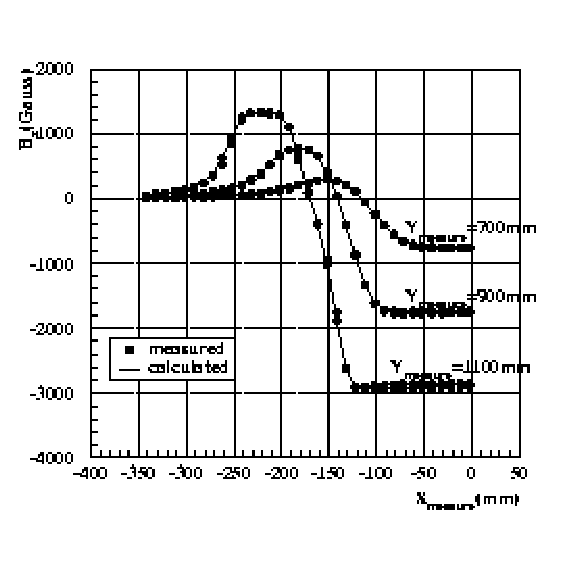
\includegraphics[bbllx=64,bblly=14,bburx=331,bbury=275,width=9.cm,height=6cm]{./figures/popField.eps}

\vspace{-5mm}

\hspace{-5mm} \includegraphics*[bbllx=340,bblly=540,bburx=650,bbury=740,width=10.5cm]{./figures/dNudB.eps}

~~~~~~~~

~~~~~~~~~

~~~~~~~~~

\end{minipage}\hspace{0mm}
\begin{minipage}[b]{.65\linewidth}
\section{\LARGE  KEK proton  machines}

\subsection*{\Large     $\bullet$ POP - Proof of principle, the first proton FFAG}
\begin{center}  First operation 2000. \end{center}
\large   
  \begin{center}
                   {\bf \Large   \underline{[Typical] data}} 
   \begin{tabular}{llccc}
\\[-3mm]
      &$E_{inj} - E_{max}$  &    keV  &     50 - 500     &             \\
      &orbit radius& m   &    0.8 - 1.14    &          \\
\multicolumn{2}{l}{\it \underline{Optics}}   \\
      & lattice    &     &  DFD    & \\
      & number of cells& &     8            &            \\
      &   K        &     &      2.5         &           \\
      &$\beta_r,~\beta_z$ max.&m  &   0.7  &        \\
      &$\nu_r~/~\nu_z$&  &    2.2~/~1.25  &   \it tunable via $B_F/B_D$ ratio        \\
%      & radial accept. & $\pi$cm &   0.4    &  \raisebox{1ex}[0mm][0mm]{\it mechanical limit is}  \\
%      &            &     &                  &  \raisebox{2ex}[0mm][0mm]{\it injection inflector}   \\[-2ex]
%      & vertical accept. & $\pi$cm &   \\
\multicolumn{2}{l}{\it  \underline{Magnet}} & &     radial sector   \\
&$\theta_D~/~\theta_F$, core&deg&   2.8~/~14      &          \\ 
      & $B_D~/~B_F$& T   &    0.04 - 0.13~/~0.14 - 0.32    &   \it  $r_{inj} \rightarrow r_{max}$       \\
      &   gap      & cm  &    30 - 9        &   \it        $gap = g_0 (r_0/r)^K$                  \\[1ex]
\multicolumn{2}{l}{\it  \underline{Injection}}& &multi- or single-turn & \bigg\{ \raisebox{1ex}[0mm][0mm]{\it electrostatic inflector} \\
      &        &         &                  &                \raisebox{2ex}[0mm][0mm]{\it  + 2 bumpers}  \\[-2ex]
\multicolumn{2}{l}{\it  \underline{Acceleration}}&&                &  \fbox{ \bf broad band, high gradient RF} \\
      & swing      & MHz &   0.6 - 1.4      &  \\
      &harmonic    &     &          1       &  \\
      &voltage p-to-p& kV&   1.3 - 3        &  \\
      & cycle time & ms  &      1       &        \fbox{  \it 1~kHz rep. rate } \\
      &   $\phi_s$ & deg &       20         &        \\
      &   $\nu_s$  &     &    0.039 - 0.012       &       \\
      &     $\dot B$ &T/s&    180        &       \\
   \end{tabular}
  \end{center}

~~~~~~~~~

~~~~~~~~~

~~~~~~~~~

\end{minipage}


%\clearpage
%\section{ POP - RF cavity} 
%\large   
%\begin{minipage}[b]{.3\linewidth}
%\hspace{-20mm} \includegraphics*[bbllx=50,bblly=50,bburx=600,bbury=470,width=9.cm]{./figures/FFAG31_cavity.eps}
%\end{minipage}\hspace{0mm}
%\begin{minipage}[b]{.65\linewidth}
%\large   
%We have developed the rf cavity, shown in Fig. 1, using two rectangular  FINEMET  cores of 
%1.1m(width) x 0.7m(height). The thickness of the core is 30mm. The window s opening is 640mm. The 
%shunt impedance of this core is about 82 ohms. The 55kW rf amplifier which consists of two tetrodes 
%(Eimac 4CW25,000) is used. 2.2 Frequency characteristic of the rf cavity. The available frequency range 
%of the whole RF system is determined by the characteristic of the impedance matching section to connect 
%the 55kW amplifier with 1kW driver amplifier, and by the choke inductance to block the rf current to the 
%anode power supply. We made a test circuit with matching transformer. In order to simulate the real condition, 
%the 200pF capacitor, which number was assumed tetrode s capacitance, was
%\end{minipage}







\clearpage


\large   

\begin{minipage}[b]{.34\linewidth}
\hspace{-20mm} \includegraphics*[bbllx=14,bblly=14,bburx=1701,bbury=1155,width=10.cm]{./figures/118-1825_IMG.eps}

``return yoke free'' magnet % (+shunt yokes)

\includegraphics*[width=7.cm]{./figures/FigTriplet.eps}

\hspace{-10mm}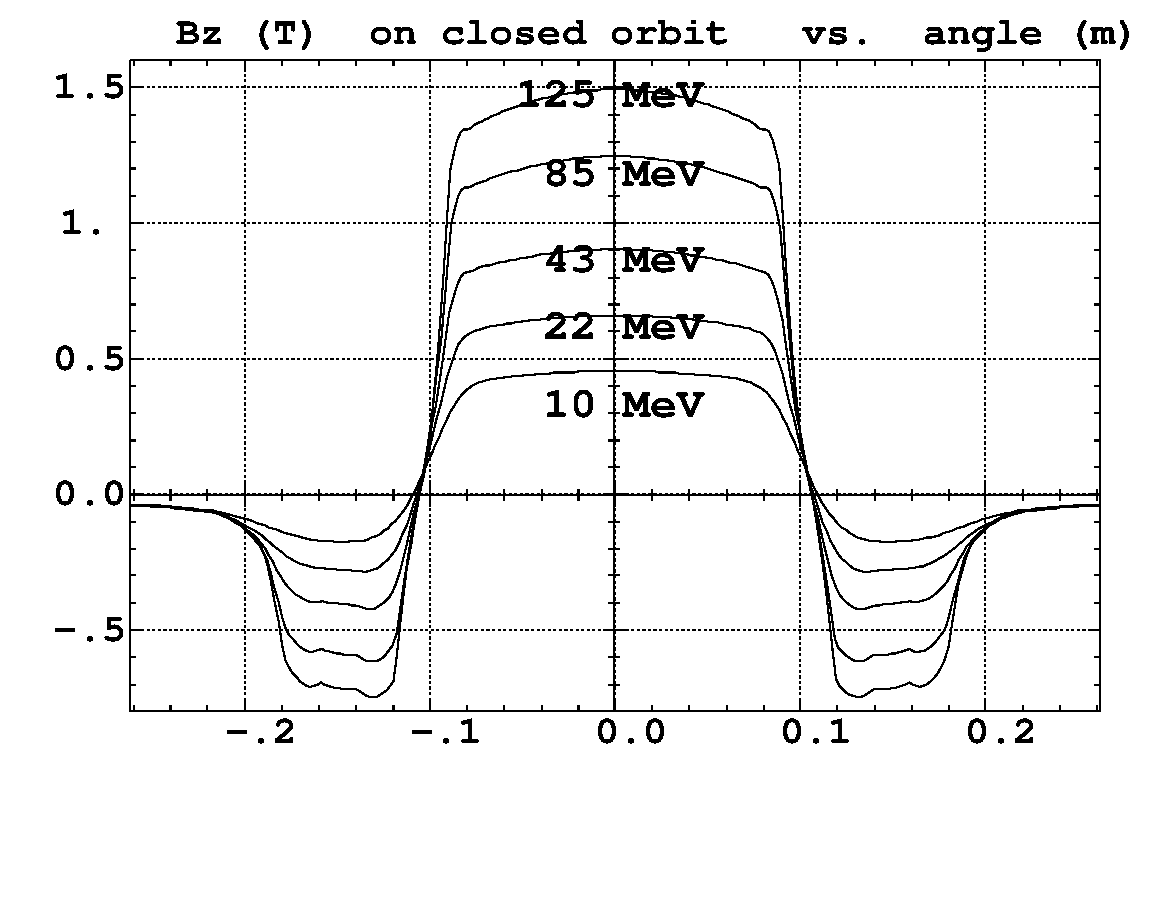
\includegraphics[bbllx=20,bblly=120,bburx=567,bbury=480,width=9.00cm,height=4cm]{./figures/fieldOnCO.eps}

\mbox{ \hspace{-20mm}
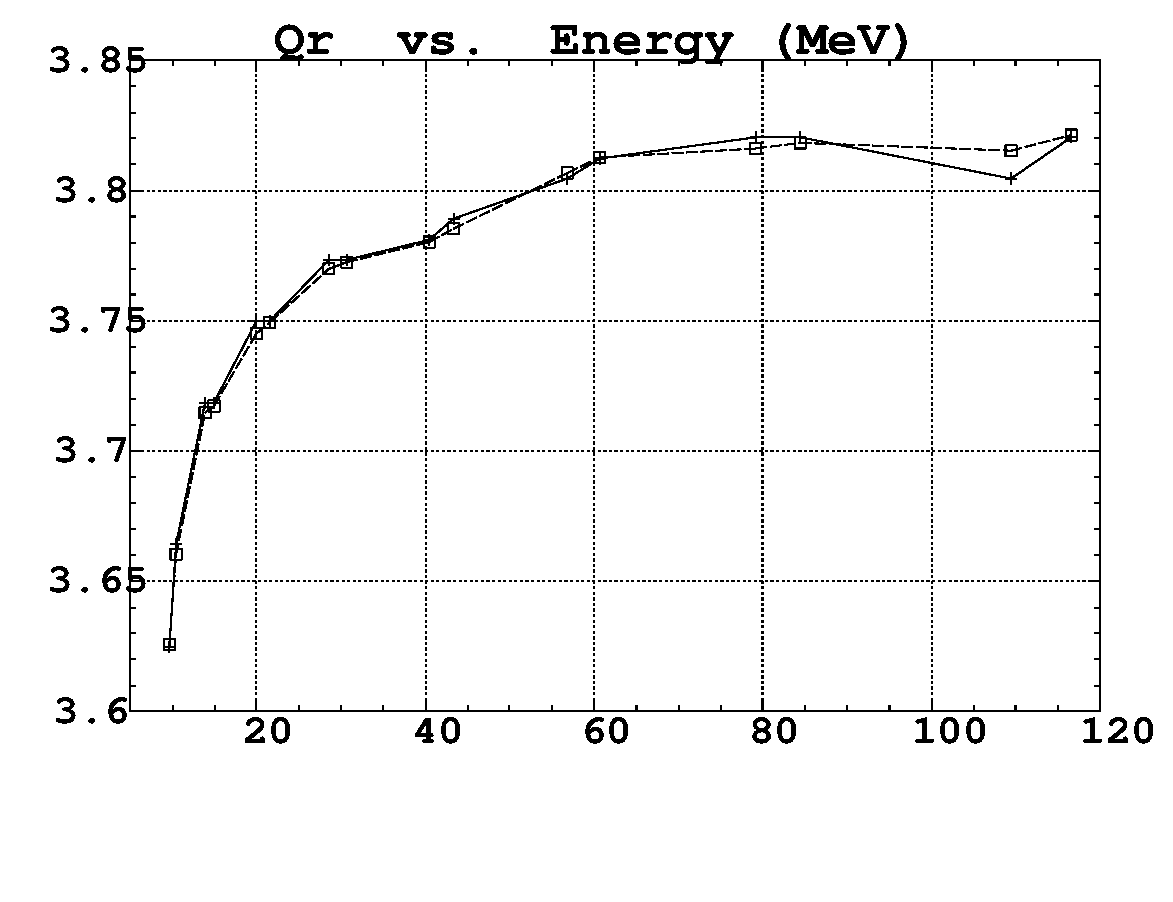
\includegraphics[bbllx=20,bblly=120,bburx=567,bbury=500,width=5.400cm]{./figures/QrVsE.eps}
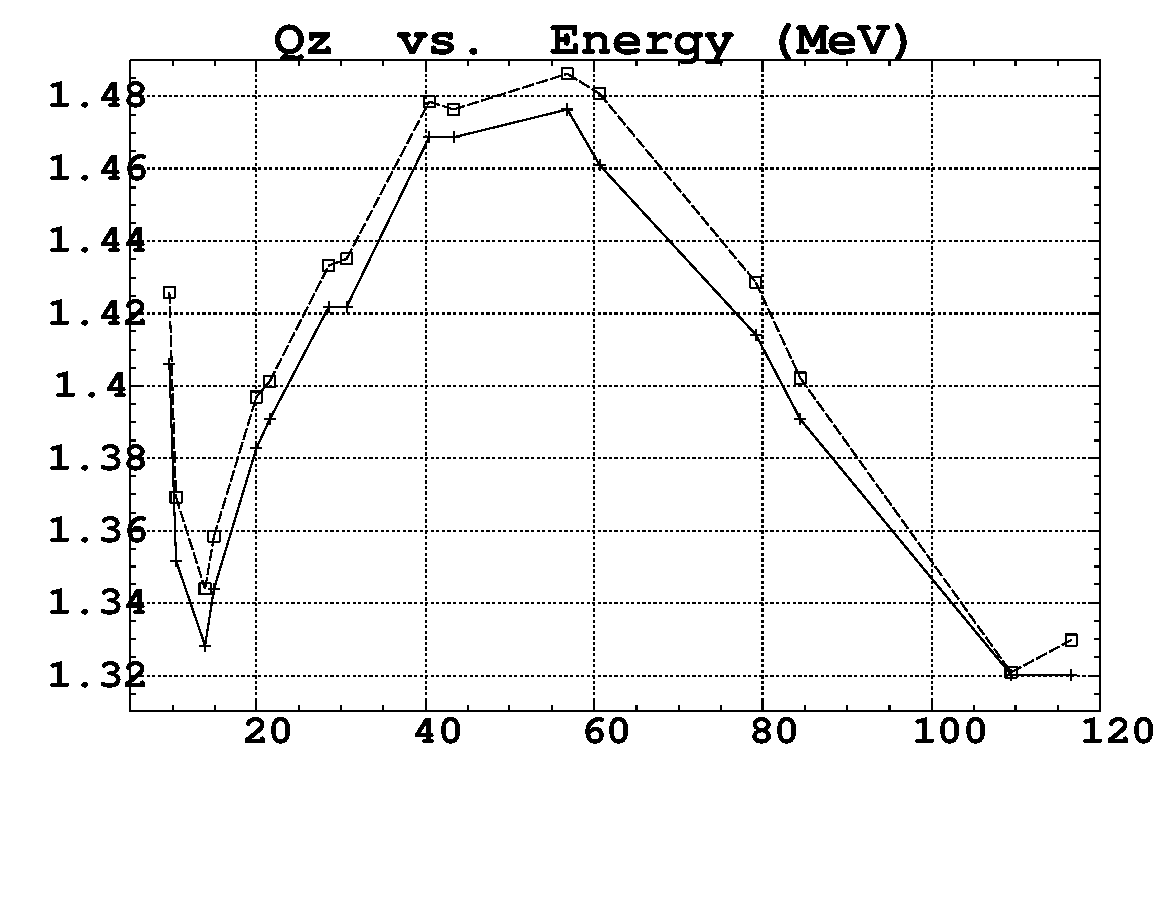
\includegraphics[bbllx=20,bblly=120,bburx=567,bbury=500,width=5.400cm]{./figures/QzVsE.eps}
}

~~~~~~~~~~~~~

\end{minipage}\hspace{0mm}
\begin{minipage}[b]{.65\linewidth}
\subsection*{\Large      $\bullet$ The 150~MeV machine}
\begin{center}  First operation 2003. \end{center}
\large   
  \begin{center}
                   {\bf \LARGE   \underline{[Typical] data}} 
   \begin{tabular}{llccc}
\\[-3mm]
      &$E_{inj} - E_{max}$  &    MeV  &     12 - 150     &             \\
      &orbit radius& m   &    4.47 - 5.20  &          \\
\multicolumn{2}{l}{\it \underline{Optics}}   \\
      & lattice    &     &   DFD     & \it 9.5~deg. drift   \\
      & numb. of cells& &      12          &            \\
      &   K        &     &      7.6         &            \\
      &$\beta_r~/~\beta_z$ max.&m  &    2.5~/~4.5  &        \\
      &$\nu_r~/~\nu_z$&  &    3.7~/~1.3  &     \it tunable via $B_F/B_D$ ratio   \\
      & $\alpha, ~ \gamma_{tr}$ &&       0.13, ~~ 2.95          & \it $1/(1+K)$, ~~ $(1+K)^{1/2}$    \\
      &  $\mathcal{R}/\rho|_{E_{max}}$ &&          5.4             \\
\multicolumn{2}{l}{\it  \underline{Magnet}}  & &               &     \it radial sector  triplet   \\
&$\theta_D~/~\theta_F$   &deg&   3.43~/~10.24    &          \\ 
      & $B_D~/~B_F$& T   &     0.2-0.78~/~0.5-1.63    &   \it $r_{inj} \rightarrow r_{max}$                \\
      &   gap      & cm  &    23.2 - 4.2        &   \it at $r_{inj}$ - $r_{max}$ ($gap = g_0 (r_0/r)^K$)      \\[1ex]
\multicolumn{2}{l}{\it \underline{Injection}}& &  multi-turn &\bigg\{  \raisebox{1ex}[0mm][0mm]{\it B-septum + E-septum}  \\
      &        &         &                  &                  \raisebox{2ex}[0mm][0mm]{\it  + 2 bumpers}  \\[-2ex]
\multicolumn{2}{l}{\it  \underline{Extraction}}& & single-turn & \it kicker + septum \\
%     & extracted emittance&$\pi$mm.mrad&      50        &         \\
\multicolumn{2}{l}{\it  \underline{Acceleration}}&&                &   \it broad band, high gradient cavity \\
      & swing      & MHz &   1.5 - 4.5      &  \\
      &harmonic    &     &          1       &  \\
      &voltage p-to-p& kV&       2        &  \\
      &   $\phi_s$ & deg &       20         &         \\
      &   $\nu_s$  &     &    0.01 - 0.0026      &       \\
      &     $\dot B$ &T/s&     300     &       \\
      &  rep. rate & Hz  &    250  \\
   \end{tabular}
  \end{center}

~~~~~~~~~~~~~~~~~~~~~~

\end{minipage}






\clearpage 

\subsection*{\Large    The design {\it must } resort to tracking}

\large   

\begin{center}  \large   

Regarding tunes, optical functions, motion stability limits, acceleration, etc., 

\bigskip

!~Things have not changed since the 50's~!  resort to field maps and tracking~: 

\bigskip

analytic and matrix approach can only yield approximate values of zero-th and first order parameters (though good enough 
as starting data for further detailed studies) 

~~~~~~~~~~~~~~~~~

~~~~~~~~~~~~~~~~~

\includegraphics*[bbllx=20,bblly=120,bburx=567,bbury=480,width=9.00cm]{./figures/FigStabLim.eps}

Acceptance  limits 

~~~~~~~~~~~~

\includegraphics*[bbllx=20,bblly=120,bburx=567,bbury=480,width=9.00cm]{./figures/analStp.06-Z1_rz.eps}

12 to 150~MeV acceleration - adiabatic damping of vertical motion. 
\end{center}






\clearpage 

\section{\LARGE After the MURA years, till 1990s}

\large     

After MURA, some actvity  went on, for instance on alternative proposals in high power proton beam based facility projects. 

\bigskip

Two examples.

\vspace{-10mm}
\begin{center}
$\bullet$ {\bf ESS}  % (S. Martin / P.F. Meads)
\end{center}

%The ESS was planned to be the European match to the American Spallation Neutron Source (SNS)
% and the Japanese Spallation Neutron Source. 
%
%\bigskip
%
%Europe has recently declared that the European Spallation Source (ESS) will not be build in the near future. 
In its latest design  ESS  accelerator facility should serve two target stations, 
one 5MW 50~Hz and the other 1MW 10Hz. 
Structure~:  a 1.33GeV H- Linac followed by 2 accumulator rings that compress the beam pulse to 0.4$\mu$s (H- 
injection, 1000 turns), 2.5MW throughput each, 2.3e14ppp, 25Hz, radius 26m, Iav in each ring=63A. 

\medskip

Alternative FFAG scheme  (early 1190's) :  0.8GeV H- Linac followed by 1.6 or 3~GeV FFAG. 

Finally rejected, considered difficult option, in particular as to injection, and high cost. 

%Intermediate FFAG design studies yielded : 
%S.~A.~Martin et als [Proc. Cycl. Conf., Vancouver (1992)]
%Specs.: 5MW beam power,  3mus pulse, 50~Hz rep. rate

\medskip

{\normalsize
   \begin{tabular}{llccl}
&beam power       &   MW  &        5                 &           \\
&top E, either    &  GeV  & 3   at $2\, 10^{14}$ppp    & . in the 1-3GeV E range, neutron flux does not depend on pBeam E \\
&          or     &       & 2   at $3\, 10^{14}$ppp    & . entails 560~MeV $E_{inj}$ and power gain of only 4       \\
&rep. rate        &   Hz  &        50                & . users' specif                         \\
&     $<I>$       &   mA  &         1.7              &     \\
&    radius       &  m    &       45                 \\
\it \large injection  &      &       &                         & .   multiturn,  charge xchange             \\
&    \# of turns      &        &         260              & .  320~$\mu$s          \\
&  circulating I &    mA  &         100              &           \\
&          E     &    MeV &         430              & . space charge tune shift constraint \\
%++ lower Ploss at injection (charge xchange,   trapping) \\
 \it \large extraction &    &        &                          & .    single turn, fast kicker      \\
&power gain with FFAG&    &        7                 & . favors lower intensity (hence higher top E and -- stronger magnets)
\\
\it \large FFAG optics   \\
&  DFD sector, ~K&        &       $21$                & . feasiblity of the magnets was demonstrated / $\gamma_{tr} > \gamma_{max}$      \\
%&   K            &        &       $21$              & . so to ensure $\gamma_{tr} > \gamma_{max}$   \\
% spiral angle   &     deg&         30               & . small, to enhance vertical focusing   \\
&   $\nu_r ~/~ \nu_z$      &        &  5.8~/~2.8        & . $\approx \sqrt{1+K}$         \\
&number of sectors&       &        20                & . to ensure smooth envelopes         \\
&$\beta_r ~/~ \beta_z max.$&\it m  &       &   \it  min-max  \\
& radial aperture&     m  &       $2.5$  &                                      \\
&  $B_{min} ~/~ B_{max}$  &  T &  -2 / 4           \\
\it\large  RF              &        &  \\
&      freq      &    MHz &       1.6-2              &             \\
&   voltage ($\times$10 cavities)&   kV  &        20                &    \\
%&    \# of cavities&      &        10                &
\end{tabular}
}




%Work related to FFAG(scaling) done in the early 90's. together with Phil Meads (Oakland).
%Phil actualy wrote the Code called ORBIT(this is not the recently developed ORBIT at BNL-SNS) calculating dynamic apertures.
%1.) SURVEY2.xls  -  a summary spread sheet of all the systems we discussed this days.
%2.) FFAGVE1.nb  -  a MATHEMATICA Note book file for fast calculation of scaled FFAG properties. I started a similar 
%program for nonscaled FFAG at Snowmass 2000, but this I  have to find in my old file mess. Sorry for the bad documentation.
%3.) Literature contains a set of references dated up to about 1994.
%I am digging out of my files a spread sheet dealing with cost estimations. This takes a little more time









\clearpage 

\begin{center}
$\bullet$ {\bf 8~GeV proton driver (FFAG03)}   % (W. Chou / P.F. Meads)
\end{center}

Option~1~:  synchrotron 

Option~2~:  Linac

Possible option~3~: FFAG, because it is supposed to feature large acceptance, high intensity, high repetition rate. 

Two optics investigated~:  spiral and radial. 

\begin{table}[h]
\begin{center}
\large 
\begin{tabular}{lcccl}
\\
             &     & \bf p-Driver& FFAG&        \\
             &     &             & radial sector  \\
\\
Energy   & GeV &     \multicolumn{2}{c}{8 }        &   . FFAG~: need more than one ring~?       \\
$E-{injection}$    & MeV &        \multicolumn{2}{c}{600}    &          \\
beam power         &  MW &     \multicolumn{2}{c}{0.5}        &   \\
 p/bunch           &     &  \multicolumn{2}{c}{$3\ 10^{11}$} &          \\
circumference      &  m  &  \multicolumn{2}{c}{$474$} &          \\
 optics            &     &                &  DFD  \\
\# of sectors      &     &                &     32 \\
  K value          &     &                &   120 \\
  radial extent    & m   &                &   4.55 \\
%\\[-3mm]
rep. rate          &     &        15      &       105        &  . $\times 7 \rightarrow$ Needs new Linac   \\
 b/pulse (RF harmonic)&  &        84      &      12          &  \\
 p/pulse           &     & $2.5\ 10^{13}$ & $3.6\ 10^{12}$   & . synchrotron  $\stackrel{1/7}{\longrightarrow} FFAG$      \\
RF frequency       & MHz &        53      &       7.5        &  . FFAG needs bunch rotation for inj. into 53~MHz MI bucket \\ 
RF peak power      & kW &      \multicolumn{2}{c}{200}       & \\
 $<I>$             &$\mu$A&    \multicolumn{2}{c}{60}        & . low beam intensity in FFAG       \\
$\beta \gamma \epsilon_{x,z}$&$10^{-6}$m.rad&\multicolumn{2}{c}{40$\,\pi$}  &        \\
$\beta \gamma \epsilon_l$& eV.s &            \multicolumn{2}{c}{0.2}  &        \\
\# of injections to MI \\
 ~ ~ ~ (inj. time 400~ms) &&      6      &        42  &  . an advantage of Option~2 compared to Option~1 \\ 
cost estimates     & M\$ &      230       &      130  & . rough, for a 0.8-2.5~GeV, 5~MW design      \\
\end{tabular}
\end{center}
\end{table}



%\clearpage
%Circular vs.Linear 
%Synchrotron: cheaper, more secure         Linac: better, more challenging 
%Strengths o 
%Natural connection to a TESLA type LC o More intense beam intensity possible o More versatile 
%physics (p, e, X-FEL) " Weaknesses o More expensive o Two critical technical issues:   1 klystron 
%driving multiple cavities   8 GeV H- injection into the MI o Difficult to use the MiniBooNE beam line 
%o To be a true  proton driver  (i.e., serving a neutrino factory), the linac needs a compressor ring. 
%" Possible improvement o To have a cost review o To carefully investigate these technical issues 
%" Strengths o A lot of the work completed - Three design iterations, all documented o More matured 
%technology ( Boring is good ) o Less expensive (TEC $230M, including 15% EDIA, 13% overhead, 30% 
%contingency) o Fit the existing complex better o Better use of Fermilab s expertise o R&D helps 
%improve the performance of existing machines " Weaknesses o Less innovative (less attractive to 
%universities) o Longer injection time to the MI " Possible improvement o To investigate ac 
%superconducting magnet technology





\clearpage 

%\addcontentsline{toc}{section}{\numberline{}\LARGE  The Neutrino Factory}
\section{\LARGE     The Neutrino Factory}

\large  
It has triggered a strong activity  in the domain of FFAG design, and lead to the development of new concepts. 

% $\theta_{1,3}$, $\Delta m_{2,3}^2$, CP violation in the lepton sector
\medskip

\begin{minipage}[b]{.43\linewidth}
\LARGE Europe NuFact\\
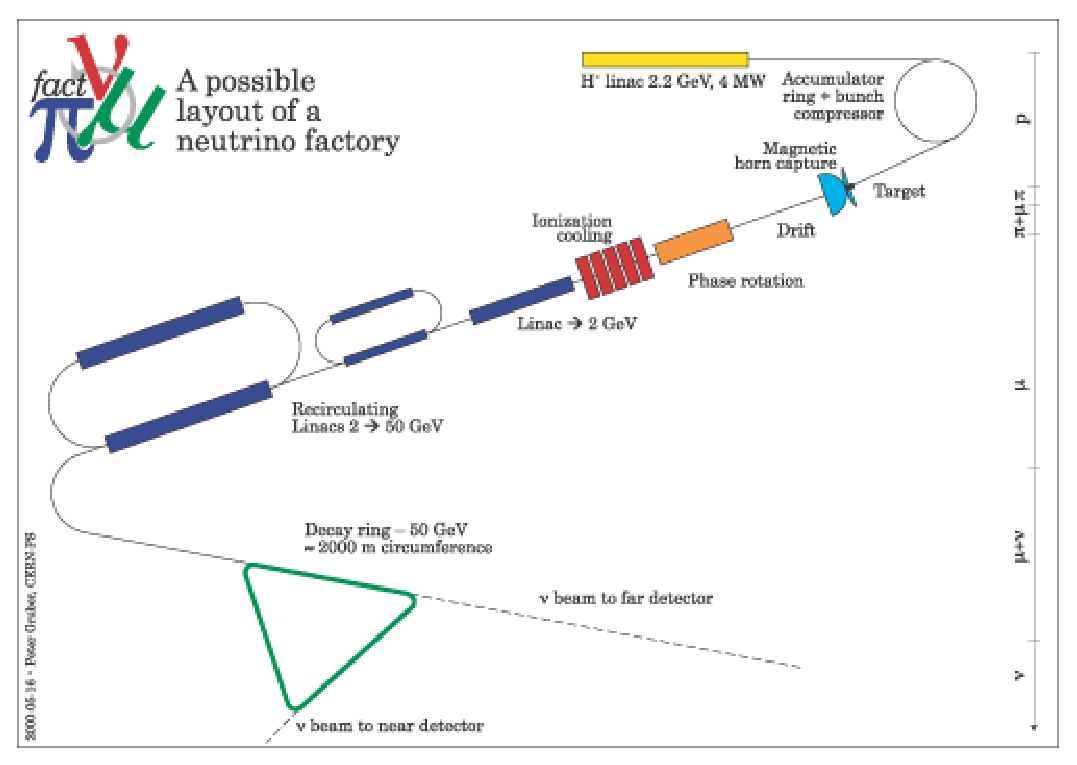
\includegraphics[bbllx=14,bblly=14,bburx=515,bbury=365,width=11cm,height=6cm]{./figures/CERN_nf_triangle.eps} \\

\vspace{-55mm}
{\footnotesize \hspace{0cm}  ~ ~ ~ ~ $A_n=1.5\pi$cm/$\pm20\%$}

\vspace{25mm}

{\footnotesize \hspace{0cm} $A_n=3\pi$cm/$\pm2\%$}
\vspace{10mm}

\rule{20mm}{.4mm}\\
\LARGE US NuFact 
\vspace{-25mm} 

\hspace{35mm}\includegraphics*[bbllx=160,bblly=30,bburx=235,bbury=280,width=2cm,angle=-90]{study-2.eps}   \\

\vspace{-10mm}
\hspace{-7mm}\includegraphics*[bbllx=0,bblly=0,bburx=263,bbury=384,width=8cm,angle=-90]{tabCost.eps}

~~~~~~~~~~~~~~

\end{minipage}\hspace{5mm}
\begin{minipage}[b]{.55\linewidth}

\large
The Europe and the two US NuFact studies propose  to  accelerate muons up to the storage energy (20 or 50~GeV) 
by means of  one or two 4- or 5-pass RLA's. RLA's are complicated machines (spreaders, combiners), hence expensive. 


\medskip

\LARGE The Japan NuFact

\large

50-GeV, $3.3\, 10^{14}$~ppp with 0.3 Hz (15~$\mu$A) ~/~ 0.75~MW

Four muon FFAG's~:  0.2-1~GeV, 1-3,  3-10 (SC),  10-20~(SC). 

No cooling, technology simpler, compact (R$\approx$200m)
\medskip

{\normalsize 30ns/300$\pm$50\%~MeV bunch } %~/~  $\approx$5~eV.s acceptance}

\vspace{-20mm}

\hspace{-1cm}\includegraphics[angle=-90,width=8cm]{./figures/g3D-gnuplot.eps}

\vspace{-6cm}
%%BoundingBox: 0 0 612 792
\includegraphics*[bbllx=100,bblly=470,bburx=660,bbury=792,width=19cm]{./figures/nuFactJ.eps2}

\normalsize 
Acceleration rate is lower than RLA, requires larger distance, but, 
acceptance is larger  both transversally (twice~: DA $3~\pi$cm norm. at $\delta p=0$) %NIMA 503 (2003) Keil 
and longitudinally ($\approx5$~eV.s). 
Hence achieve comparable production rate~:   $\approx 10^{20}$ muon decays per year (1~MW p power). 
\end{minipage}\hspace{0mm}



\clearpage 


%All in all, now admitted :  
%same rate of 0.3 muons per proton incident on target  attained with both NuFact designs, RLA and FFAG. 

\begin{minipage}[b]{.65\linewidth}

\section*{\Large Non-scaling designs}

\begin{center}
A new concept has developed since late 90's, with muon activities~:  

{\bf \LARGE ``linear, non-scaling optics'': 

 FFAG  based on linear optical elements  

tunes  are allowed to  vary with orbit}


\end{center}

\medskip

This has a series of consequences~: 

   $\bullet$ yields large DA  $\leftarrow$ fields are linear - prone to allow less cooling

   $\bullet$ small $\delta$TOF over  energy span, allows high frequency / high gradient RF

   $\bullet$  $R/\rho<2$ - this decreases the {\Large$\mu$} decay loss

   $\bullet$ horizontal beam excursion is reasonable $\rightarrow$ reasonable apertures

\bigskip

In practice, the cell tune is allowed to decrease from just below a half-integer value at injection, to just 
above the lower integer. 

- hence tens of cells cause Xing of tens of  integer and  $\frac{1}{2}$integer resonances. 

- yet the {\bf crossing is fast}, this should result in not too stringent tolerance on alignements and field defects.  


~~~~~~~~

Above 5~GeV, non-scaling linear  FFAG  yield  lower cost/GeV than RLA. 

\vspace{4cm}

Proposed FFAG scheme of a  NuFact~: 
\medskip

\fbox{\Large \bf from cooling/pre-acceleration 
$\rightarrow$ dogbone RLA $[ 2$-$5~$GeV$] \rightarrow$  FFAG $[ 5$-$10~$GeV$] \rightarrow$   FFAG $[ 10$-$20~$GeV$]$  } 


~~~~~~~~

\end{minipage}\hspace{0mm}
\begin{minipage}[b]{.65\linewidth}

{\bf \large ~ ~  ~ ~ ~ 6-20~GeV lattices, $314$~cells,  

~ ~  ~ ~ ~ C$\approx$2~km, B$<$6~T, B'$<$80 T/m  

~ ~ ~ ~ ~ ~   9~MV RF per cell, \fbox{5 turns}
}

\mbox{
\includegraphics*[bbllx=20,bblly=120,bburx=567,bbury=480,width=4.600cm]{./figures/fodoCell.eps}
\includegraphics*[bbllx=20,bblly=120,bburx=567,bbury=480,width=4.600cm]{./figures/cell.eps}
}

{\normalsize ~ ~ ~ FODO (QF-O-BD-O)  ~ ~  FDF (O-QF-BD-QF-O)}

\mbox{
\includegraphics*[bbllx=20,bblly=100,bburx=567,bbury=480,width=4.600cm]{./figures/clorbParab.eps}
\includegraphics*[bbllx=20,bblly=100,bburx=567,bbury=480,width=4.600cm]{./figures/dC.eps}
}

{\large ~ ~  $x_{co}\in [-8,+8]$~cm ~ ~ ~ ~ ~  $\delta$TOF$<3\, 10^{-4}$  }

\mbox{
\includegraphics*[bbllx=20,bblly=100,bburx=567,bbury=480,width=4.600cm]{./figures/tunes.vs.E.eps}
\includegraphics*[bbllx=20,bblly=100,bburx=567,bbury=480,width=4.600cm]{./figures/betvsp.eps}
}

{\large  Cell tunes: $0.5^-\rightarrow .1^+$ ~~   Optical functions}


%\vspace{-4cm} \hspace{5cm}
 ~ ~ ~ ~ ~  ~ ~ ~~  \includegraphics*[angle=-90,width=4.400cm]{./figures/cavite200.eps}

{\large ~ ~ ~ ~ ~ ~ ~ ~ ~  200~MHz RF  Cavity }


~~~~~~~~~~~~~~

~~~~~~~~~~~~~~

~~~~~~~~~~~~~~

\end{minipage}\hspace{0mm}






\clearpage 

\section*{\LARGE An e-model of a muon FFAG}

\large 

``Since no non-scaling FFAG has ever been built, there is interest in building a small model which would accelerate 
electrons and demonstrate our understanding of non-scaling FFAG design. `` 
 [Review of Current FFAG Lattice Studies in North America, JS Berg et als, 2004]

\bigskip

\begin{minipage}[b]{.45\linewidth}
\large 
\begin{tabular}{lcccl}
Energy             &\it MeV &    10 to 20    \\
number of turns    &        &     5 to 11    \\
circumference      &\it  m  &       17       &   \\
 lattice           &\it     &       FDF      \\
tune variation     &\it     &  $<$0.5        \\
 number of cells   &\it     &       45       &   \\
 cell length       &\it  m  &     0.38       &   \\
RF drift  length   &\it cm  &       10       \\       
\it CF magnets: \\
- length F/D  &\it cm  &     5 / 10     &      \\
- field  F/D  &\it  G  &    375 / 107   & \\
- gradient F/D&\it T/m &      6 / -5    & \\
- apertures   &\it cm  & 1.2$\times$1.8 & \\
alignement tolerances &  &                &  \\
gradient tolerances&        &                &  \\
length variation   &\it rel.&  $2\ 10^{-3}$  &       \\
RF frequency       &\it GHz &        3       &  \\
peak RF voltage    &\it kV  &       $<$80    &   \\
     $h$           &        &        171     &   \\ %number of bunches up to $h$ \\
RF power           &\it kW  &      $<$1.5  \\
 max. I  (beam loading)& mA &      100       
\end{tabular}

~~~~~~~~~~~~~~~~~

~~~~~~~~~~~~~~~~~

~~~~~~~~~~~~~~~~~

\end{minipage}\hspace{10mm}
\begin{minipage}[b]{.65\linewidth}

\includegraphics*[bbllx=14,bblly=14,bburx=271,bbury=271,width=12cm]{./figures/emodelBeta.eps}

%\includegraphics*[bbllx=14,bblly=14,bburx=273,bbury=167,width=9cm]{./figures/emodelResoXing.eps}

\end{minipage}\hspace{0mm}





\end{document}












\clearpage


\addcontentsline{toc}{subsection}{\numberline{}\Large  Low-energy beta-beam}
\subsection*{\Large  Low-energy beta-beam}


\includegraphics[width=20cm,angle=-90]{betaBFacility.eps}





\clearpage

\subsection{\Large  Eu collaboration in the field}


\begin{minipage}[b]{.55\linewidth}
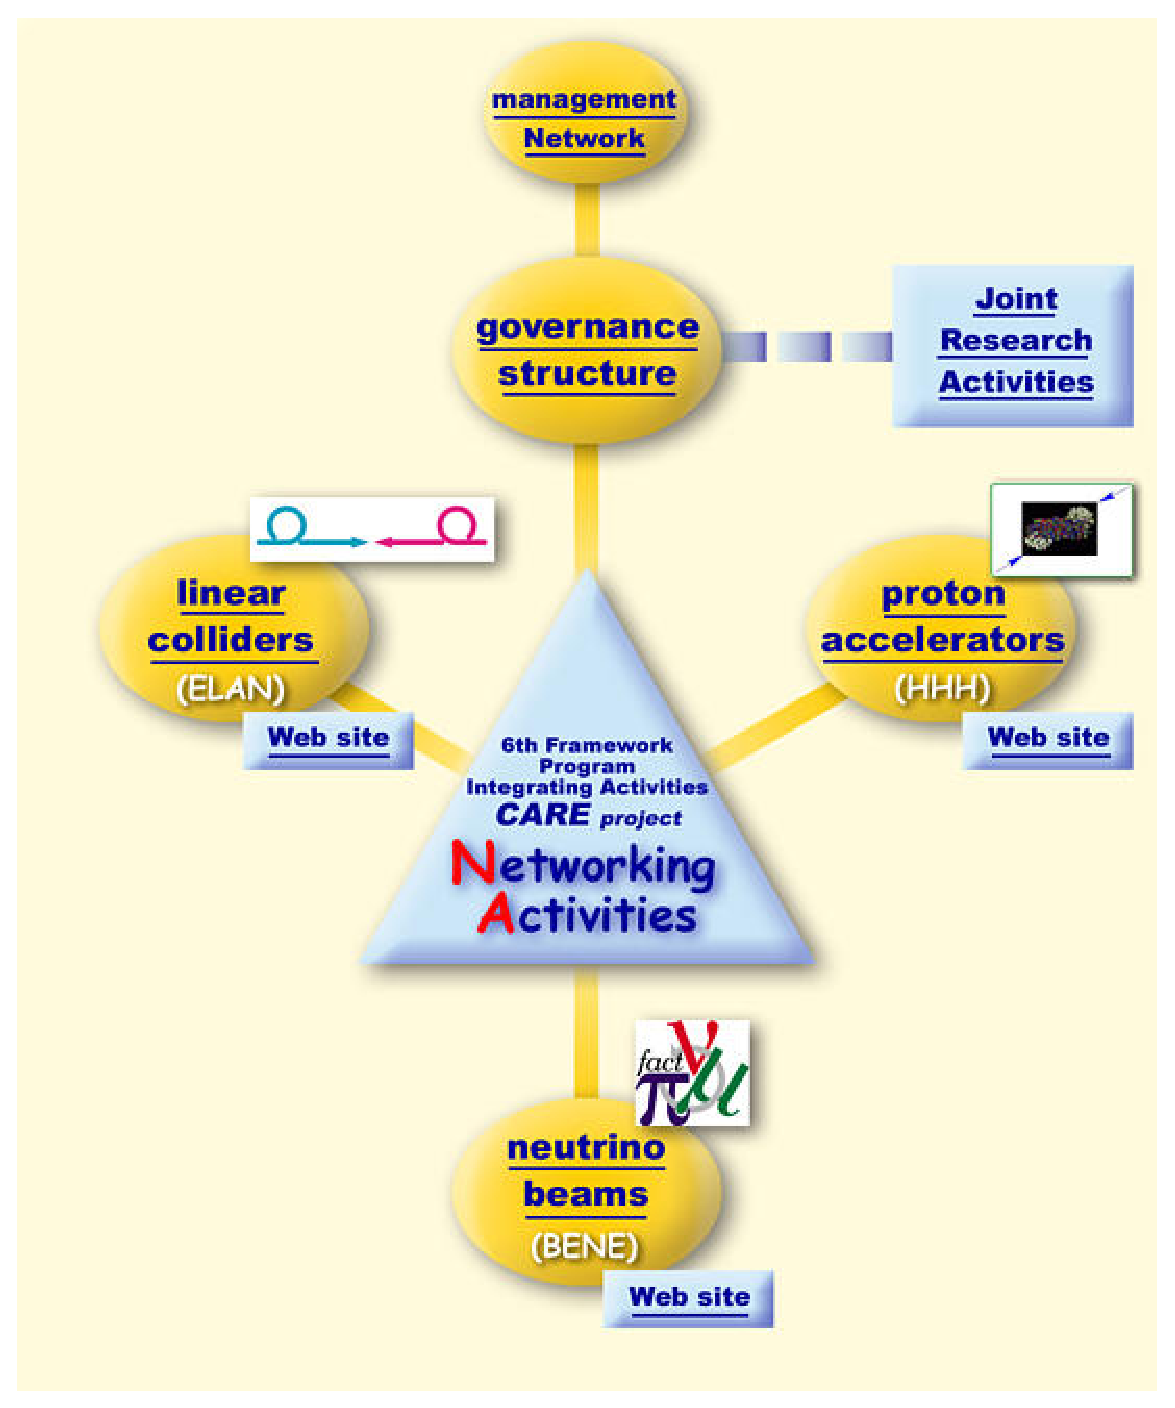
\includegraphics[width=14cm]{./figures/current-na-half.eps}
\end{minipage}\hspace{0mm}
\begin{minipage}[b]{.55\linewidth}
\normalsize \rm 

Mostly Structured in the frame of CARE/BENE Networking Activity (http://BENE.na.infn.it/) \\
(Beams for European Neutrino Experiment) 

Participation in world collaboration (J+US)~: workshops, video meetings, etc. 

\smallskip
\bf BENE/WP5(MuEnd) team~: \rm

~~~~~~~~~~\\
* Bruno Autin CERN AB/ABP   \\
- low beta FFAG optics for cooling  \\
* Stephen Brooks, RAL   \\
- capture, compression,  cooling ring, acceleration in isoChr. FFAG   \\
Jean-Marie De Conto CNRS, IN2P3, Grenoble    \\
Denis De Menezes CEA DAPNIA, Saclay    \\
* Olivier Delferri`ere CEA DAPNIA, Saclay    \\
- magnets for quadrupole decay channel   \\
Jie Gao CNRS, LAL, Orsay    \\
* Eberhard Keil, Berlin   \\
- e-model, optics and parameters - with A. Sessler   \\
* Franck Lemuet, CERN AB/LEI   \\
- decay channel and FFAG acceleration   \\
* Fran�ois M\'eot CEA DAPNIA  \& CERN (associate)   \\
- tracking  tools and optics studies \\
Mauro Migliorati INFN - Lab. Naz. di Frascati    \\
Luigi Palumbo INFN - Lab. Naz. di Frascati    \\
* Jaroslaw Pasternak, CERN AB/ABP   \\
- cooling ring   \\
* Jacques Payet CEA DAPNIA, Saclay    \\
- RLA optics   \\
* G. Rees, RAL   \\
- see S Brooks. Isochr. ring   \\
*  Horst Schonauer \\
- muon cooling  in FFAG   \\
Bruno Spataro INFN - Lab. Naz. di Frascati    \\
Franco Tazzioli INFN - Lab. Naz. di Frascati    \\
* Andr\'e Verdier CERN AB/ABP   \\
- MAD+PTC tool for FFAG design   
\end{minipage}



%\subsection{\Large  The structure of world  collaboration in the field}
%World DS planned. 
%Objective~: ``Study III''. FFAG based. 









******* Questions
Only 5 FFAG machines  operated~:     check that
 $\approx 10^{21}$ muons per year. verifier
Given that the time of flight spread in scaling ffag is large, how does the RF track the accelerated beam?
 the optics (tunes, etc.) is the same, whatever the orbit $r$ :      a preciser...

\subsection*{\Large     201~MHz RF cavity for non-scaling FFAG}



\centerline{\bf \large   Transverse acceptance in the Linac}
\centerline{--------------}

\large   
Basis hypothesis are the characteristics of the 220~MHz  cavity, as extrapolated 
from the Cornell/CERN cavity. Typical~: 

$\lambda_{RF}$ = 1.3627m, \,\,\,\, pipe radius = 0.18m.
\begin{figure}[h]
\begin{center}
\includegraphics[height=12cm,width=8cm,angle=90]{cavite200.eps}
\end{center}
\end{figure}






